
\documentclass[12pt,aspectratio=169]{beamer}

% Packages
\usepackage{mathtools}
\usepackage{hyperref}
\usepackage{setspace}
\usepackage{tikz}
\usetikzlibrary{positioning}
\usepackage{ragged2e}
\usepackage{nicematrix}
\usepackage[compatibility=false]{caption}
\usepackage[framemethod=tikz]{mdframed}

% Colored boxes
\usepackage{tcolorbox}
\tcbsetforeverylayer{autoparskip} % Removes unwanted vertical space

% Theme
\usetheme{metropolis}
\metroset{subsectionpage=progressbar,sectionpage=none}
\setbeamertemplate{theorems}[numbered]

\usepackage{fontspec}
\defaultfontfeatures{LetterSpace=30}


% Code
\usepackage{listings}
% Custom colors
\definecolor{codegreen}{rgb}{0,0.6,0}
\definecolor{codegray}{rgb}{0.5,0.5,0.5}
\definecolor{codepurple}{rgb}{0.58,0,0.82}
\definecolor{backcolour}{rgb}{0.95,0.95,0.92}
\definecolor{light-gray}{gray}{0.95}
% Python style for highlighting
\newcommand\pythonstyle{\lstset{
		backgroundcolor=\color{white},
		language=Python,
		basicstyle=\ttfamily\footnotesize,
		morekeywords={self},              % Add keywords here
		keywordstyle=\color{blue},
		stringstyle=\footnotesize\color{deepgreen},
		commentstyle=\color{codegreen},
		showstringspaces=false,
		frame=tb,
		numbers=left,
		numbersep=5pt,
		numberstyle=\tiny\color{gray},
		columns=fullflexible,
		numbersep=5pt,
		aboveskip=1em,
		showtabs=false,
		tabsize=2,
		gobble=3
	}}

% Python environment
\lstnewenvironment{python}[1][]
{
	\pythonstyle
	\lstset{#1}
}
{}
% Python for inline
\newcommand\pythoninline[1]{{\pythonstyle\lstinline!#1!}}

% Tables and justification
\newcommand{\ra}[1]{\renewcommand{\arraystretch}{#1}}
\justifying

% Subfigures
\setbeamertemplate{caption}[numbered]
\usepackage[caption=false,font=footnotesize]{subfig}

% Colors
\setbeamercolor{uppercolgreen}{fg=white,bg=green!35}
\setbeamercolor{lowercolgreen}{fg=black,bg=green!10}
\setbeamercolor{uppercolred}{fg=white,bg=red!35}
\setbeamercolor{lowercolred}{fg=black,bg=red!10}
\setbeamercolor{uppercolblue}{fg=white,bg=blue!35}
\setbeamercolor{lowercolblue}{fg=black,bg=blue!10}
\definecolor{darkred}{rgb}{0.55, 0.0, 0.0}
\definecolor{darkpastelblue}{rgb}{0.47, 0.62, 0.8}
\definecolor{darkcerulean}{rgb}{0.03, 0.27, 0.49}
\definecolor{darkgreen}{rgb}{0.0, 0.55, 0.0}
\definecolor{deepblue}{rgb}{0,0,0.5}
\definecolor{deepred}{rgb}{0.6,0,0}
\definecolor{deepgreen}{rgb}{0,0.5,0}

% Matrix size
\usepackage{stackengine}
\stackMath
\def\sss{\scriptstyle \color{gray}}
\setstackgap{L}{12pt}
\def\stacktype{L}

% Mathematical commands
\newcommand{\vc}[1]{\boldsymbol{\mathbf{#1}}}
\newcommand{\pr}[1]{{#1\,}'}
\newcommand{\idx}[2]{{\color{darkpastelblue}[}#1{\color{darkpastelblue}]_{#2}}}
\newcommand{\shape}[2]{\stackunder{#1}{\sss #2}}
\DeclareMathOperator*{\argmax}{arg\,max}
\DeclareMathOperator*{\argmin}{arg\,min}

% Style commands
\newcommand{\myalert}[1]{{\color{darkred}\textbf{#1}}}

% White frame (for images)
\newenvironment{whiteframe}[1]{
	\setbeamercolor{background canvas}{bg=white}
	\begin{frame}{#1}
		}{
	\end{frame}
}

\setbeamerfont{frametitle}{size=\normalsize}
\setbeamertemplate{frametitle}[default][right]
{
}
%\setbeamercolor{frametitle}{fg=white,bg=black!75}

% No headline frame
\makeatletter
\newenvironment{noheadline}{
	\setbeamertemplate{headline}{}
	\addtobeamertemplate{frametitle}{\vspace*{-3.5\baselineskip}}{}
}{}
\makeatother

% Lists
\setbeamertemplate{itemize items}[triangle]

% Footnotes
\setbeamertemplate{footnote}%
{%
	\parindent 1.5em\noindent%
	\justifying\setstretch{0.7}%
	\hbox to 1em{\hfil\insertfootnotemark}\begin{scriptsize}\insertfootnotetext\end{scriptsize}\par%
}

% Footnote without number
\newcommand\blfootnote[1]{%
	\begingroup
	\renewcommand\thefootnote{}\footnote[frame]{\noindent#1}%
	\addtocounter{footnote}{-1}%
	\endgroup
}

% Theorems
\newcommand*{\theorembreak}{\usebeamertemplate{theorem end}\framebreak\usebeamertemplate{theorem begin}}
\newcounter{theo}[section]\setcounter{theo}{0}
\renewcommand{\thetheo}{\arabic{section}.\arabic{theo}}

\newenvironment{theo}[2][]{%
	\refstepcounter{theo}%
	\ifstrempty{#1}%
	{\mdfsetup{%
			frametitle={%
					\tikz[baseline=(current bounding box.east),outer sep=0pt]
					\node[anchor=east,rectangle,fill=red!10]
					{\strut Theorem~\thetheo};}}
	}%
	{\mdfsetup{%
			frametitle={%
					\tikz[baseline=(current bounding box.east),outer sep=0pt]
					\node[anchor=east,rectangle,fill=red!10]
					{\strut Theorem~\thetheo:~#1};}}%
	}%
	\mdfsetup{innertopmargin=5pt,linecolor=red!10,%
		linewidth=2pt,topline=true,%
		frametitleaboveskip=\dimexpr-\ht\strutbox\relax
	}
	\begin{mdframed}[]\relax%
		\label{#2}}{\end{mdframed}}

% The 2024 source used annotate-equations for two optional visual labels.
% Keep the equations portable in the 2026 repository when that package is absent.
\newcommand{\eqnmarkbox}[3][]{#3}
\newcommand{\annotate}[4][]{}

% Colors
\definecolor{titlecolor}{RGB}{245, 242, 238} 
\definecolor{drawgray}{HTML}{666666}
\definecolor{drawgray_l}{HTML}{F5F5F5}
\definecolor{drawblue}{HTML}{6C8EBF}
\definecolor{drawblue_l}{HTML}{DAE8FC}
\definecolor{drawgreen}{HTML}{82B366}
\definecolor{drawgreen_l}{HTML}{D5E8D4}
\definecolor{draworange}{HTML}{D79B00}
\definecolor{draworange_l}{HTML}{FFE6CC}
\definecolor{drawyellow}{HTML}{D6B656}
\definecolor{drawyellow_l}{HTML}{FFF2CC}
\definecolor{drawred}{HTML}{B85450}
\definecolor{drawred_l}{HTML}{EA6B66}
\definecolor{drawviolet}{HTML}{9673A6}
\definecolor{drawviolet_l}{HTML}{E1D5E7}

\begin{document}

	{\usebackgroundtemplate{\tikz\node[opacity=0.4,inner sep=0]{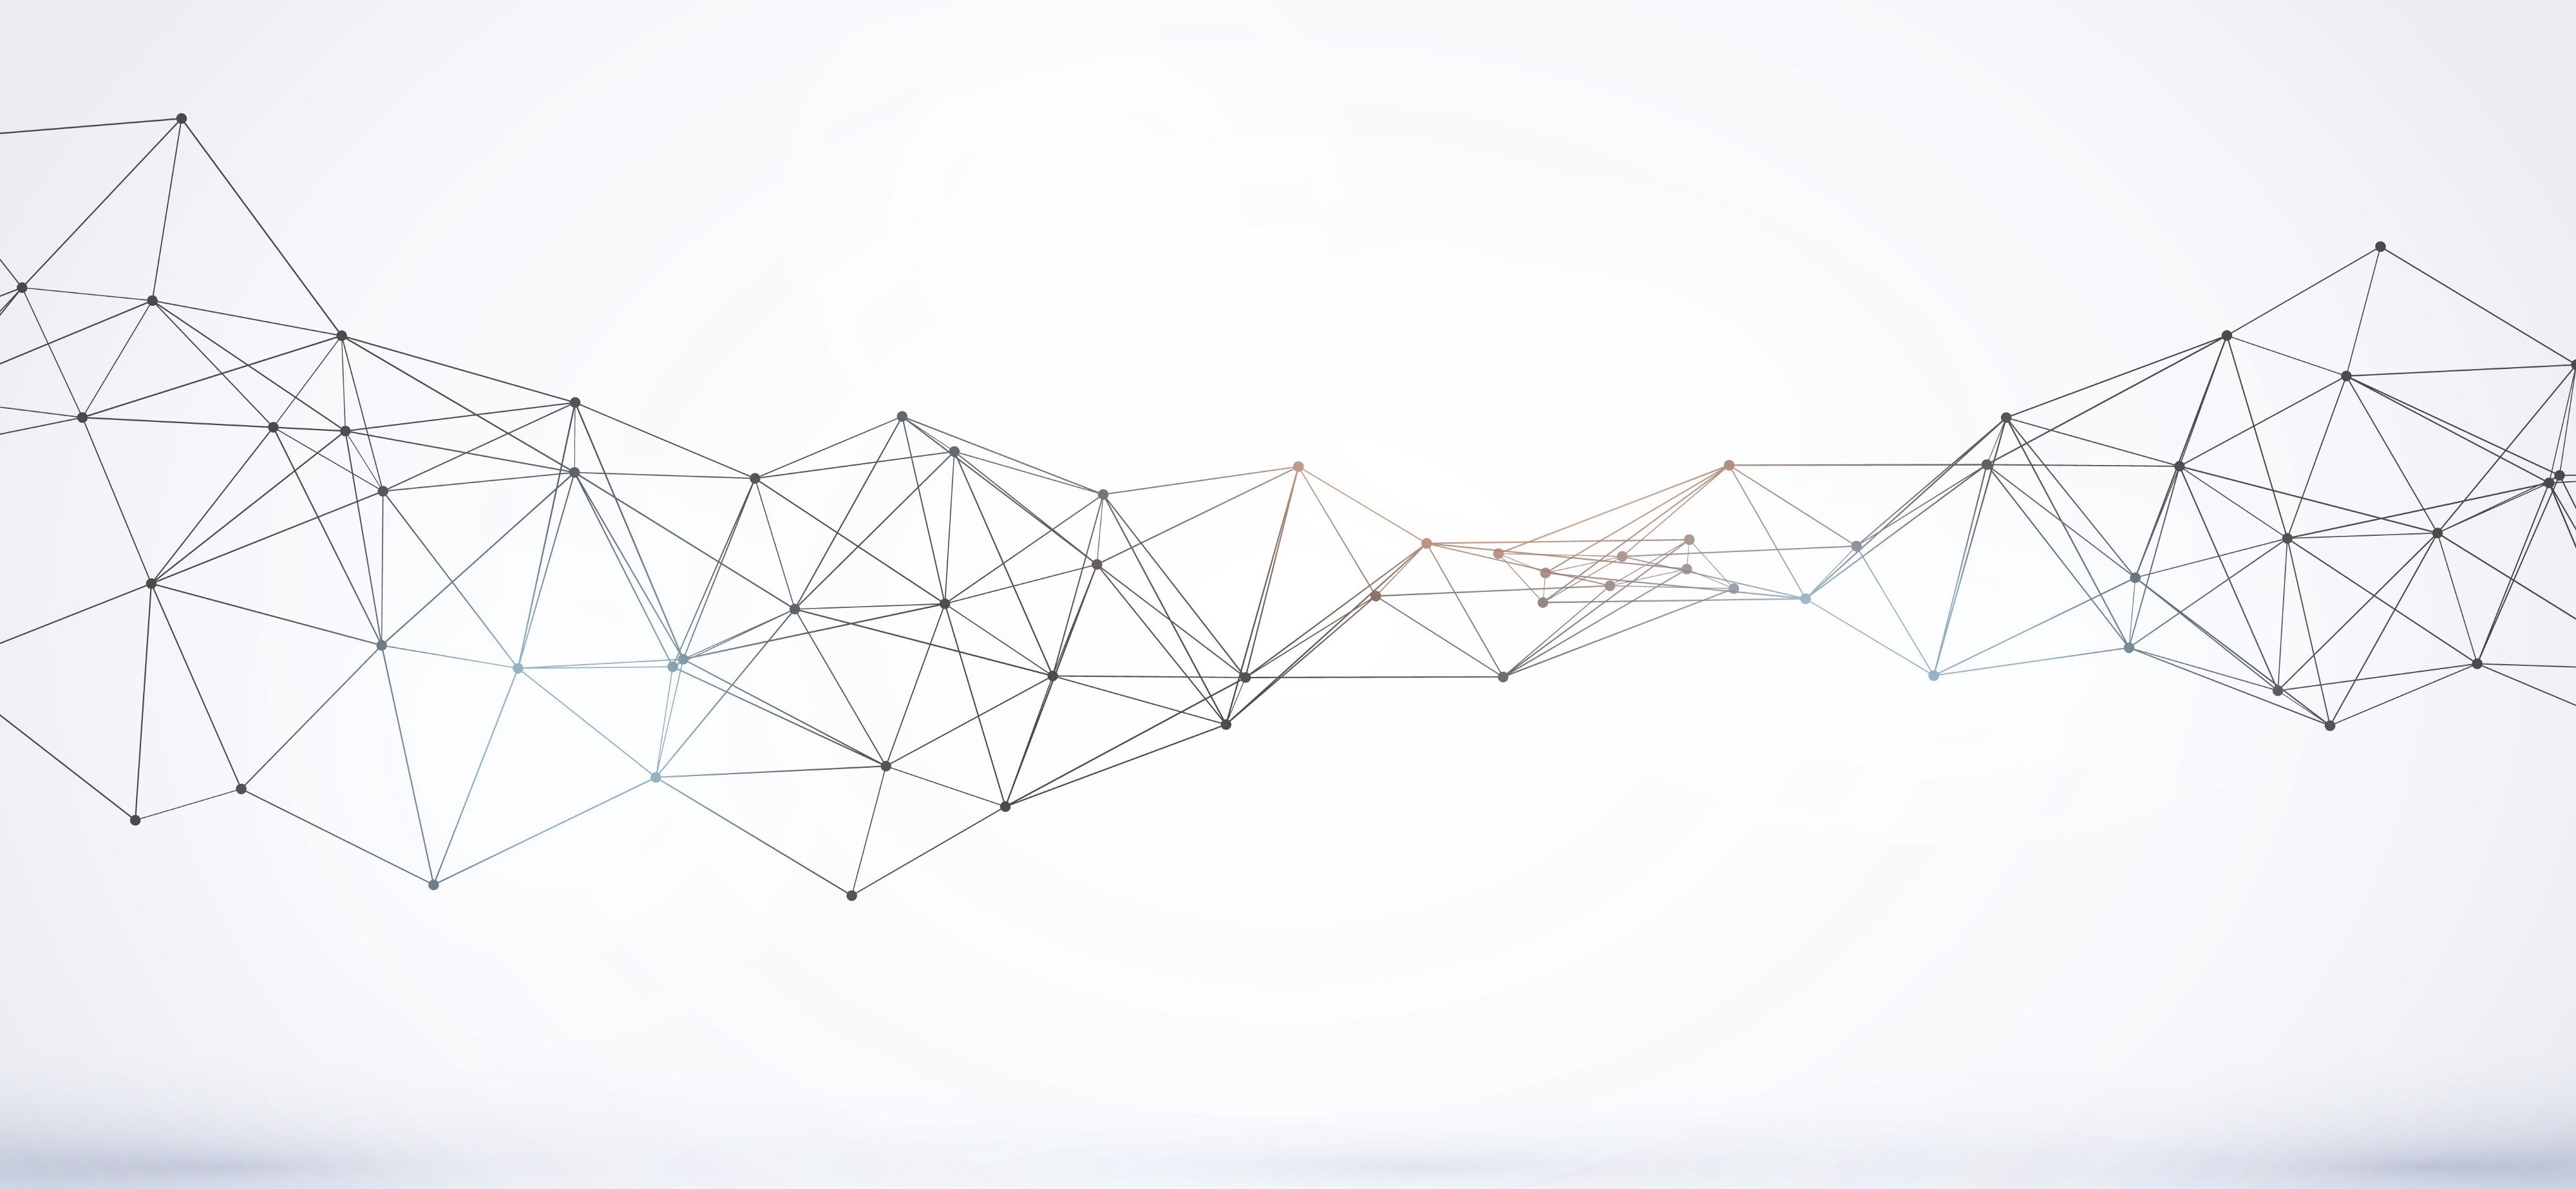
\includegraphics[width=\paperwidth,height=\paperheight]{images/header}};}%
	\begin{frame}[plain]
		\vspace{0.5cm}
		\title{\large \begin{spacing}{1.0}Neural Networks for Data Science\end{spacing}\vspace{0.25em}
			\normalsize \begin{spacing}{1.0}\textbf{Master's Degree in Data Science}\end{spacing}\vspace{0.5em}}
		\subtitle{\Large \textbf{Lecture 2: Mathematical preliminaries}\\
		\large 2b. Mathematical optimization}
		\date{
			{
\includegraphics[scale=0.8]{images/Uniroma1}}
		}
		\author{
			\setlength{\tabcolsep}{2pt}
			\begin{tabular}{rl}
				\textbf{Lecturer}: & S. Scardapane \\
			\end{tabular}
		}\titlepage
	\end{frame}
	}

\section{Derivatives and gradients}
\subsection{Derivatives and gradients}

\begin{frame}{Empirical risk minimization}
	
	For a batch of examples $\left\{x_i, y_i\right\}_{i=1}^B$ (more on this next lecture), let $\boldsymbol{\theta}$ denote the trainable parameters of a model $f_{\boldsymbol{\theta}}(x)$ (e.g., for a linear layer $\boldsymbol{\theta}=\{\vc{W},\vc{b}\}$) and define:
	%
	\begin{equation}
		\mathcal{L}(\boldsymbol{\theta}) =
		\frac{1}{B}\sum_{b=1}^{B}
		\ell\Bigl(f_{\boldsymbol{\theta}}(x_b),y_b\Bigr)\,.
	\end{equation}
	%
	where $\ell$ is some per-example loss. Training is the optimization problem:
	%
	\begin{equation*}
		\boldsymbol{\theta}^* = \argmin_{\boldsymbol{\theta}}\mathcal{L}(\boldsymbol{\theta})\,.
	\end{equation*}
	
\end{frame}

\begin{frame}{Derivative}
	
	Most of this course is funded upon the notion of derivative.
	
	\begin{tcolorbox}
		The \myalert{derivative} of a function $f(x)$ is defined as:
		%
		\begin{equation}
			\partial f(x) = \frac{\partial}{\partial x}f(x) = \pr{f}(x) = \lim_{h \rightarrow 0} \frac{f(x+h) - f(x)}{h} \,.
		\end{equation}
		%
		Even for a continuous function, $\partial f(x)$ might not be defined everywhere.
	\end{tcolorbox}

	Informally, the derivative expresses the rate of change of $f$ around an infinitesimal displacement from $x$, or the slope of the line tangent to $f(x)$.
	
\end{frame}

\begin{frame}{Examples of derivatives}
	
	Derivative of a polynomial:
	%
	\[
		\partial \left[ x^p \right] = px^{p-1} \,.
	\]
	
	Derivative of exponentials and logarithms:
	%
	\begin{gather*}
		\partial \left[ \exp(x) \right] = \exp(x) \,, \\
		\partial \left[ \log(x) \right] = \frac{1}{x} \,.
	\end{gather*}
	
\end{frame}

\begin{whiteframe}{Visualizing derivatives in the 1D case}
		
	\begin{figure}
	\centering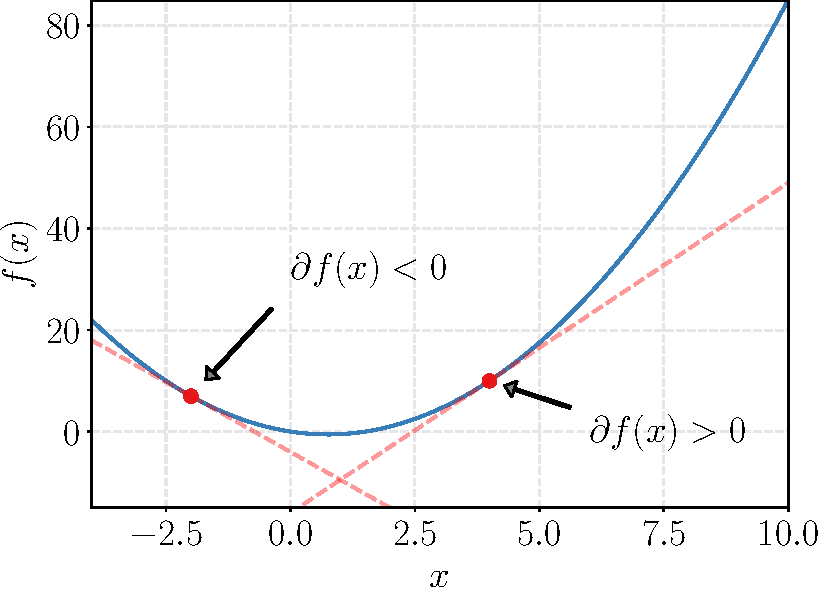
\includegraphics[width=8cm,keepaspectratio]{images/lecture_2/gradient_info.pdf} %
	\caption{1D function ($f(x) = x^2 - 1.5x$), showing the derivative at two different locations.}
	\end{figure}
		
\end{whiteframe}

\begin{frame}{Properties of derivatives}
	
	Derivatives possess a number of properties, most notably:
	%
	\begin{itemize}
		\item \textbf{Linearity}: $$ \partial \Big[{\color{darkred}f(x)} + {\color{darkgreen}g(x)}\Big] = {\color{darkred}\pr{f}(x)} + {\color{darkgreen}g'(x)} \,. $$
		\item \textbf{Product rule}: $$ \partial\Big[ {\color{darkred}f(x)}{\color{darkgreen}g(x)}\Big] = {\color{darkred}\pr{f}(x)}{\color{darkgreen}g(x)} + {\color{darkred}f(x)}{\color{darkgreen}g'(x)} \,, $$
		\item \textbf{Chain rule} $$ \partial \Big[{\color{darkred}f(}{\color{darkgreen}g(x)}{\color{darkred})}\Big] = {\color{darkred}\pr{f}(}{\color{darkgreen}g(x)}{\color{darkred})}{\color{darkgreen}g'(x)} \,. $$
	\end{itemize}		

\end{frame}

\begin{frame}{Gradient}
	
	For a function $y=f(\vc{x})$, $\vc{x} \in \mathbb{R}^m$, the \myalert{gradient} $\partial f(\vc{x})$ is an $m$-dimensional vector defined as:%
	\begin{equation}
		\idx{\partial f(\vc{x})}{i} = \frac{\partial y}{\partial \vc{x}} = \lim_{h \rightarrow 0} \frac{f(\vc{x} + h\vc{e}_i) - f(\vc{x})}{h} \,,
	\end{equation}
	%
	where $\vc{e}_i$ is the $i$th standard basis vector:
	%
	\begin{equation*}
		\idx{\vc{e}_i}{j} = \begin{cases} 1 & \text{ if } i=j \\ 0 & \text{otherwise} \end{cases}
	\end{equation*} 
	%
	Sometimes we use the alternative notation $\nabla f(\vc{x})$.
	
\end{frame}

\begin{frame}{Directional derivative}
	
	\begin{tcolorbox}
	More generally, the \myalert{directional derivative} of $f(\vc{x})$  in the direction $\vc{v}$ is:
	%
	\begin{equation}
		\mathrm{D}_{\vc{v}}f(\vc{x}) = \lim_{h \rightarrow 0} \frac{f(\vc{x} + h\vc{v}) - f(\vc{x})}{h} \,,
	\end{equation}
	\end{tcolorbox}
	%
	It is easy to prove that:
	%
	\begin{equation}
		\mathrm{D}_{\vc{v}}f(\vc{x}) = \langle \nabla f(\vc{x}), \vc{v} \rangle \,.
	\end{equation}
	%
	A partial derivative is a directional derivative in the direction of a standard basis vector.

\end{frame}

\begin{frame}{Gradients and Jacobians}
	
	Everything extends to vector-valued functions $\vc{y} = f(\vc{x})$, $\vc{x} \in \mathbb{R}^m$, $\vc{y} \in \mathbb{R}^n$:
	%
	\begin{tcolorbox}
		The \myalert{Jacobian} $\stackunder{\partial f(\vc{x})}{\sss (n, m)}$ of $f$ is a matrix defined as:
		%
		\begin{equation}
			\partial f(\vc{x}) = \begin{pmatrix}
				\frac{\partial y_1}{\partial x_1} & \dots & \frac{\partial y_1}{\partial x_m} \\
				\vdots & \ddots & \vdots \\
				\frac{\partial y_n}{\partial x_1} & \dots & \frac{\partial y_n}{\partial x_m} \\
			\end{pmatrix} \,.
		\end{equation}
	\end{tcolorbox}
	%
	For $n=1$, we recover the gradient, while for $m = n = 1$ we recover the standard derivative.
	
\end{frame}

\begin{frame}{Examples of matrix derivatives}
	
	Derivative of the inner product:
	%
	\[
	\frac{\partial}{\partial \vc{x}} \langle \vc{x}, \vc{y} \rangle = \vc{y} \,.
	\]
	
	Derivative of a linear map:
	%
	\[
	\frac{\partial}{\partial \vc{x}} \vc{A}\vc{x} = \vc{A} \,.
	\]
	
	Derivative of a norm:
	%
	\[
	\partial \lVert \vc{x} \rVert^2 = 2\vc{x} \,.
	\]
	
	\blfootnote{See the matrix cookbook for reference: \\ \url{https://www.math.uwaterloo.ca/~hwolkowi/matrixcookbook.pdf}.}
	
\end{frame}

\begin{frame}{Properties of the gradients}
	
	Jacobians inherit many properties from the scalar case. Importantly, there exists a chain rule for Jacobians. For $f: \mathbb{R}^m \rightarrow \mathbb{R}^n$ and $g: \mathbb{R}^o \rightarrow \mathbb{R}^m$:
	%
	\begin{equation}
		\stackunder{\partial \left[ f(g(x)) \right]}{\sss (n,o)} = \stackunder{\partial f(\bullet)}{\sss (n,m)} \; \stackunder{\partial g(x)}{\sss (m,o)} \,.
	\end{equation}
	%
	In words: the Jacobian of the composition of two functions is the product of their Jacobian matrices.
	
\end{frame}

\begin{frame}{First-order approximation}
	
	Given a function $f(\vc{x}_0)$ evaluated at $\vc{x}_0$, then the function:
	
	\vspace{1em}
	$$
	\widetilde{f}(\mathbf{x})= f(\mathbf{x}_0)+\langle \eqnmarkbox[drawred]{node}{\partial f(\mathbf{x}_0)}, \eqnmarkbox[drawgreen]{node2}{\mathbf{x}-\mathbf{x}_0} \rangle
	\annotate[yshift=1em]{above,right}{node}{Slope of the line}
	\annotate[yshift=-1em]{below,left}{node2}{Displacement from $\mathbf{x}_0$}
	$$
	\vspace{1em}
	
	is the best \textbf{linear approximation} of $f$ around $\vc{x}_0$ (\myalert{Taylor's theorem}). Better approximations can be constructed from higher-order derivatives, but this is enough for building effective optimization algorithms.
	
\end{frame}

\begin{whiteframe}{Visualizing the approximation}
	
	\begin{figure}
		\centering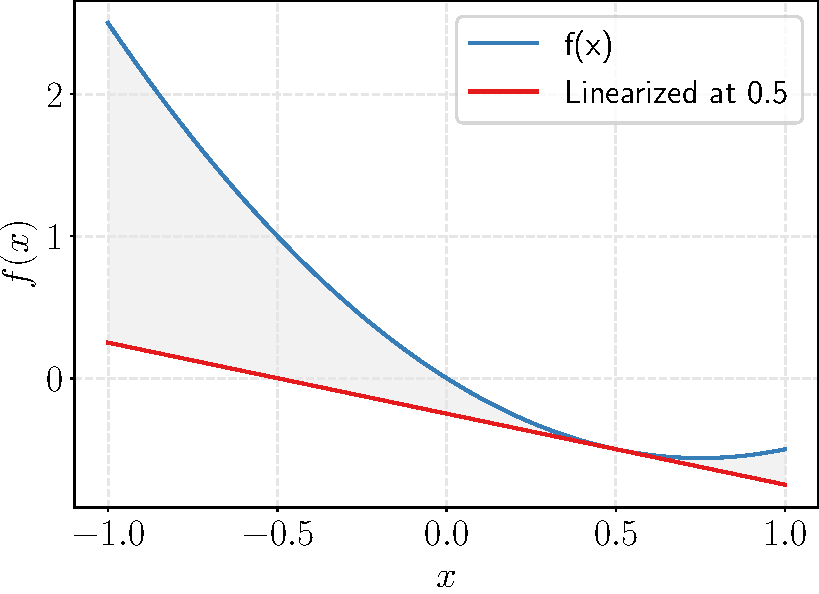
\includegraphics[width=8cm,keepaspectratio]{images/lecture_2/taylor_approximation.pdf} %
		\caption{1D function ($f(x) = x^2 - 1.5x$), linearized at 0.5.}
	\end{figure}
	
\end{whiteframe}

%\begin{frame}{Taylor's theorem (with remainders)}
%	
%	Taylor's theorem is sometimes shown in an alternative form, which is useful for proofs and for optimization:
%	%
%	\begin{equation}
%		f(\vc{x} + \underbrace{\alpha\vc{h}}_{\mathclap{\text{Small displacement along } \vc{h}}}) = f(\vc{x}) + \alpha \langle \partial f(\vc{x} + \widetilde{\alpha}\vc{h}), \vc{h} \rangle \,,
%	\end{equation}
%	%
%	for some \textit{unknown} $\widetilde{\alpha} \in \left[0, \alpha\right]$. Note that there is no approximation in the result, provided the neighbourhood is sufficiently small.
%	
%	\begin{tcolorbox}
%	\textbf{Important corollary}: if $\langle \partial f(\vc{x}), \vc{h} \rangle < 0$, for suitably small $\alpha$, then $f(\vc{x} + \alpha\vc{h}) < f(\vc{x})$ ($\vc{h}$ is a \myalert{descent direction}).
%	\end{tcolorbox}
%
%\end{frame}

\subsection{Numerical optimization}

\begin{frame}{Optimizing a function}
	
	We can use gradients to solve generic problems of the form:
	%
	\begin{equation}
		\boldsymbol{\theta}^* = \argmin_{\boldsymbol{\theta}} \mathcal{L}(\boldsymbol{\theta}))
	\end{equation}
	%
	Note that maximizing/minimizing are equivalent in the sense that:
	%
	\begin{equation}
		\boldsymbol{\theta}^* = \argmax_{\boldsymbol{\theta}} \mathcal{L}(\boldsymbol{\theta}) = \argmin_{\boldsymbol{\theta}} {\color{darkred} -} \mathcal{L}(\boldsymbol{\theta})
	\end{equation}

\end{frame}

\begin{frame}{A few additional definitions}
	
	\begin{tcolorbox}
		A point $\boldsymbol{\theta}$ such that $\mathcal{L}(\boldsymbol{\theta}) \le \mathcal{L}(\boldsymbol{\theta}') \;\;\forall\; \boldsymbol{\theta}'$ is called a \myalert{global minimum}. If instead (less restrictive):
		%
		\begin{equation}
			\mathcal{L}(\boldsymbol{\theta}) \le \mathcal{L}(\boldsymbol{\theta}') \;\;\forall\; \boldsymbol{\theta}' \in \left\{ \boldsymbol{\theta}': \lVert \boldsymbol{\theta}' - \boldsymbol{\theta} \rVert^2 < \varepsilon \right\}
		\end{equation}
		%
		for some $\varepsilon > 0$, it is called a \myalert{local minimum}.
	\end{tcolorbox}
	
	\begin{tcolorbox}
		If $\nabla \mathcal{L}(\boldsymbol{\theta}) = 0$, $\boldsymbol{\theta}$ is called a \myalert{stationary point}. Stationary points can be minima, maxima, or inflection points (aka \myalert{saddle points}).
	\end{tcolorbox}

	In general, gradient optimization can find stationary points (mostly local minima, as saddle points are escaped due to numerical noise).
	
\end{frame}

\begin{whiteframe}{Types of stationary points}
		
	\begin{figure}
	\centering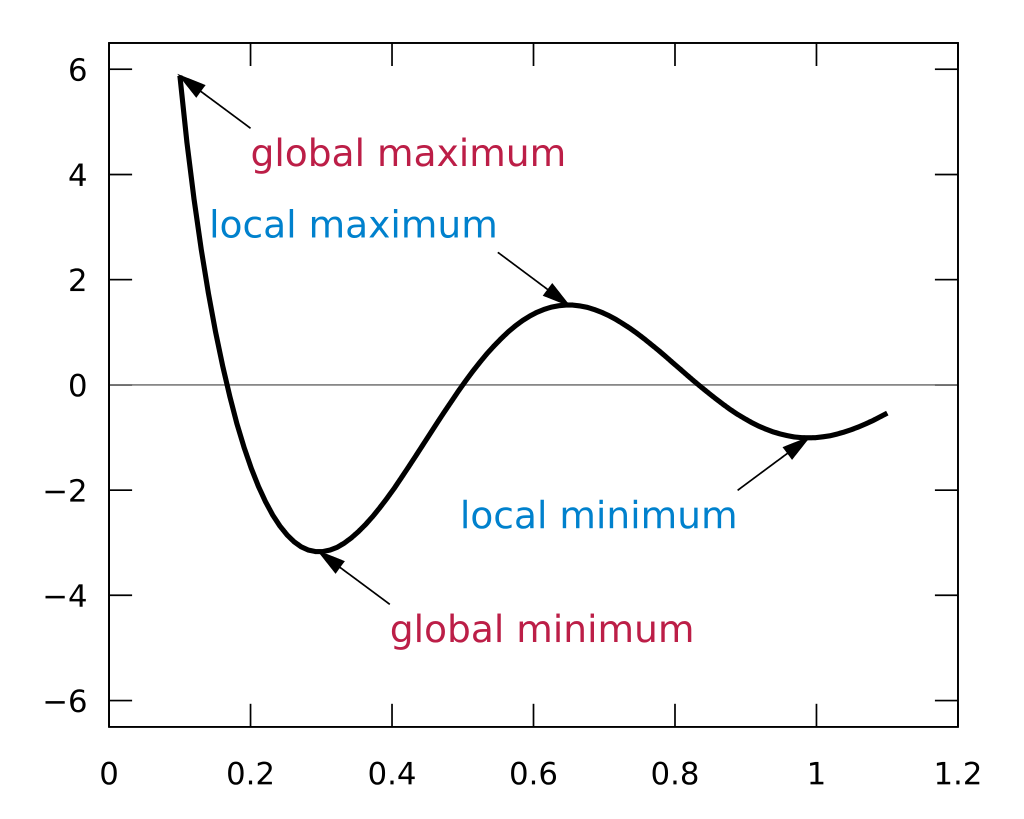
\includegraphics[width=8cm,keepaspectratio]{images/lecture_2/Extrema_example_original.png} %
	\vspace{-1em}\caption{With no additional information, stationary points can be \myalert{minima}, \myalert{maxima}, and can be \myalert{local} or \myalert{global} (\textit{Wikimedia, KSmrq}).}
	\end{figure}
		
\end{whiteframe}

\begin{whiteframe}{Saddle points}
		
	\begin{figure}
	\centering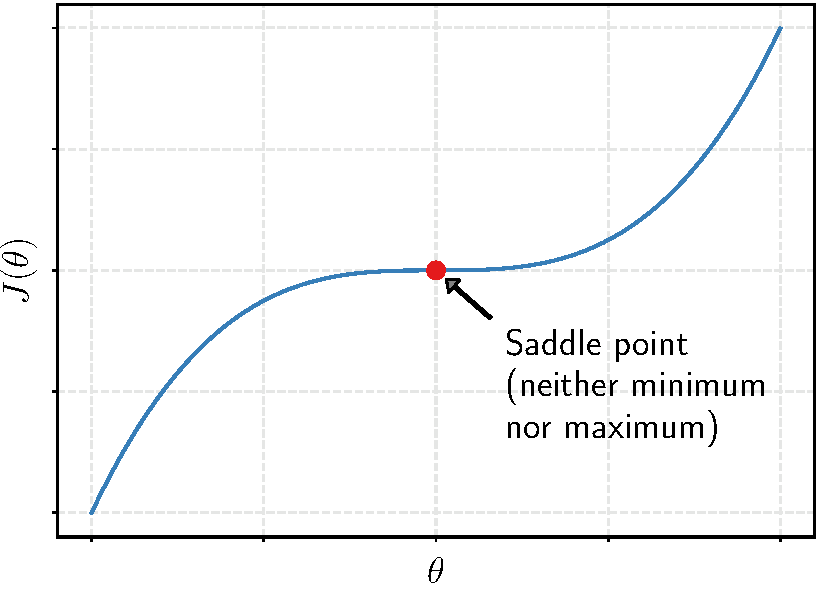
\includegraphics[width=8cm,keepaspectratio]{images/lecture_2/saddle_point.pdf} %
	\vspace{-0.5em}\caption{Stationary points can also be \myalert{saddle points}, either decreasing or increasing in different directions.}
	\end{figure}
		
\end{whiteframe}

\begin{frame}{Finding stationary points}
	
	Given a randomly initialized $\boldsymbol{\theta}_0$, consider the following iteration:
	
	\vspace{1em}
	\begin{equation}
		\boldsymbol{\theta}_t = \eqnmarkbox[drawred]{node}{\boldsymbol{\theta}_{t-1}} + \eqnmarkbox[drawblue]{node2}{\eta_t\mathbf{p}_t}
		\label{eq:iterative_descent}
		\annotate[yshift=1em]{above,left}{node}{Guess at iteration $t$}
		\annotate[yshift=-1em]{below,left}{node2}{Displacement at iteration $t$}
	\end{equation}
	\vspace{1em}

	\begin{tcolorbox}
		$\vc{p}_t$ is called a \myalert{descent direction} for $\mathcal{L}(\boldsymbol{\theta}_{t-1})$ if $\mathcal{L}(\boldsymbol{\theta}_t) < \mathcal{L}(\boldsymbol{\theta}_{t-1})$ for a sufficiently small $\eta_t$. $\eta_t$ is called \myalert{step size} or \myalert{learning rate}.
	\end{tcolorbox}
	
	To implement this iterative algorithm we need a way to choose a descent direction (and a step size) for all $t$.

\end{frame}

\begin{frame}[fragile]{Descent direction}
	
	Without lack of generality, we restrict to unit directions ($\lVert \vc{p}_t \rVert = 1$). The rate of change is given by the directional derivative:\blfootnote{We rely on the identity $\langle \vc{a}, \vc{b} \rangle = \lVert \vc{a} \rVert \lVert \vc{b} \rVert \cos(\theta)$ for vectors $\vc{a}, \vc{b}$ and angle $\theta$ between them.}
	%
	\begin{equation*}
		\mathrm{D}_{\vc{p}_t} \mathcal{L}(\boldsymbol{\theta}_{t-1}) = \langle \nabla \mathcal{L}(\boldsymbol{\theta}_{t-1}), \vc{p}_t \rangle = \lVert \nabla \mathcal{L}(\boldsymbol{\theta}_{t-1}) \rVert \underbrace{\lVert \vc{p}_t \rVert}_{=1} \cos(\theta) = \lVert \nabla \mathcal{L}(\boldsymbol{\theta}_{t-1}) \rVert \cos(\theta).
	\end{equation*} 
	%
	The above quantity is minimized when $\cos(\theta) = -1$, which happens if $\theta=\pi$, i.e., $\vc{p}_t = - \nabla \mathcal{L}(\boldsymbol{\theta}_{t-1})$. This is the \myalert{steepest descent direction}. In general, anything with $\cos(\theta) < 0$ is a descent direction.
	
\end{frame}

\begin{frame}{Gradient descent}
	
	The resulting algorithm is called \myalert{gradient descent}.
	%
	\begin{tcolorbox}
		Gradient descent (GD) finds stationary points by iterating:
		%
		\begin{equation}
		\boldsymbol{\theta}_t = \boldsymbol{\theta}_{t-1} - \eta_t \nabla \mathcal{L}(\boldsymbol{\theta}_{t-1}) \,.
	\end{equation}
	\end{tcolorbox}

	This is the basic form of gradient descent (GD, also known as \textbf{first-order} optimization): steepest local directions are not necessarily the \textit{fastest} in general and we can accelerate this iteration in many ways.
	
\end{frame}

\begin{frame}{Handling large datasets}
	
	Consider the steps needed for a single iteration of GD in our specific optimization problem:
	
	\begin{enumerate}
		\item Computing the output of the model $f(\vc{x})$ on \textit{all} examples;
		\item Computing the gradient of the cost function with respect to the parameters.
	\end{enumerate}
	
	Both these operations scale \textit{linearly} in the number of examples, which is unfeasible when we have $10^5$ or even more examples.
	
	In practice, to train neural networks we use \myalert{stochastic} versions of GD, that approximate the real gradient from smaller amounts of data.
	
\end{frame}

\begin{frame}{Stochastic GD}
	
	The key observation is that the training problem in NNs is an expectation with respect to all data ($\vc{\theta}$ is the set of weights):
	%
	\begin{equation}
		J(\vc{\theta}) = \frac{1}{n} \sum_{i=1}^n \displaystyle \ell(y_i, f_{\boldsymbol{\theta}}(x_i)) \,.
	\end{equation}
	
	To limit the complexity, we can use only a \myalert{mini-batch} $\mathcal{B}$ of $M$ examples randomly sampled from the full dataset:
	%
	\begin{equation}
		J(\vc{\theta}) \approx \widetilde{J}(\vc{\theta}) = {\color{darkred}\frac{1}{M} \sum_{i \in \mathcal{B}}} \displaystyle \ell(y_i, f_{\vc{\theta}}(x_i))\,.
	\end{equation}
	%
	The mini-batch gradient is a (unbiased, noisy) estimate of the full gradient.
	
\end{frame}

\begin{frame}{Characteristics of stochastic GD}
	
	The previous algorithm is called \myalert{stochastic gradient descent} (SGD).
	
	The computational complexity of an iteration of SGD is fixed with respect to $M$ (the \myalert{batch size}) and does not depend on the size of the dataset.
	
	If we assume that elements of the dataset are i.i.d., we can prove that SGD also converges to a stationary point \textit{in average}, albeit \textit{with noisy steps}.
	
\end{frame}

\begin{whiteframe}{Visualization of the loss}
	
	\begin{figure}
		\centering
		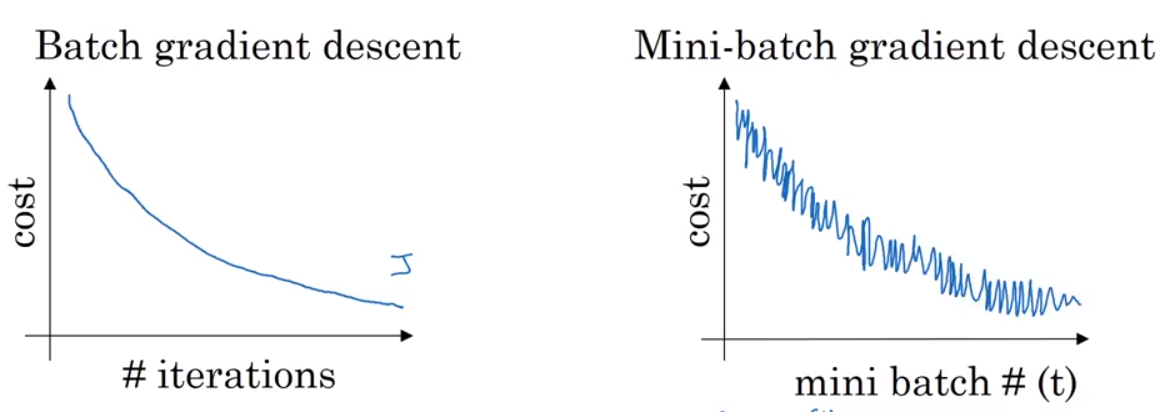
\includegraphics[width=0.9\columnwidth]{images/lecture_2/stochastic_loss_descent.png}
		\caption{SGD will converge on average to a stationary point, although in an apparently noisy fashion (Source: \href{https://engmrk.com/mini-batch-gd/}{EngMRK}).}
	\end{figure}
	
\end{whiteframe}

\begin{frame}{Extracting batches from the data}
	
	Instead of randomly sampling batches from the training dataset at each iteration, we generally apply the following procedure:
	
	\begin{enumerate}
		\item Shuffle the full dataset;
		\item Split the dataset into blocks of $M$ elements and process them sequentially, batch-by-batch;
		\item After the last block, return to point (1) and iterate.
	\end{enumerate}
	
	A full pass over the dataset is called an \myalert{epoch}. This is efficient because the majority of the time we deal with data stored \textit{contiguously} in memory. In practice, even the shuffling operation can be approximated.
	
\end{frame}

\begin{whiteframe}{Extracting batches from the data}
	
	\begin{figure}
		\centering
		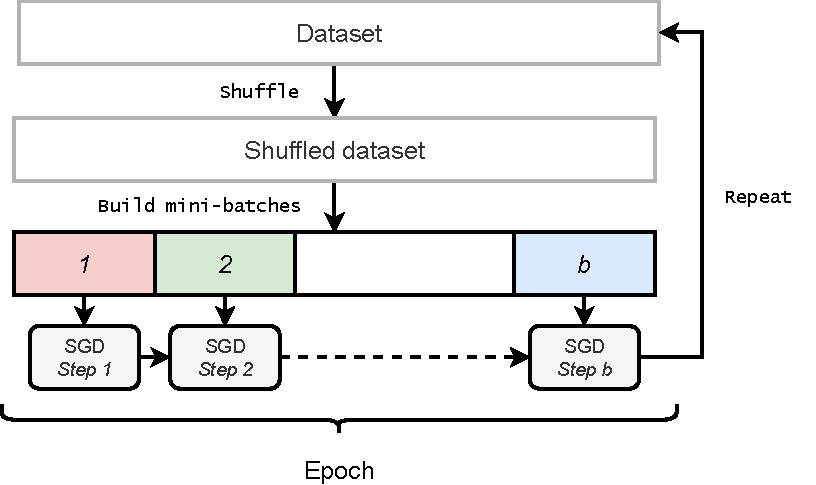
\includegraphics[width=0.75\columnwidth]{images/lecture_2/stochastic_optimization.pdf}
		\caption{Dividing the optimization process into epochs is also helpful to define metrics and stopping criteria.}
	\end{figure}
	
\end{whiteframe}

\begin{whiteframe}{Parallelizing GD optimization}
	
	\begin{figure}
		\centering
		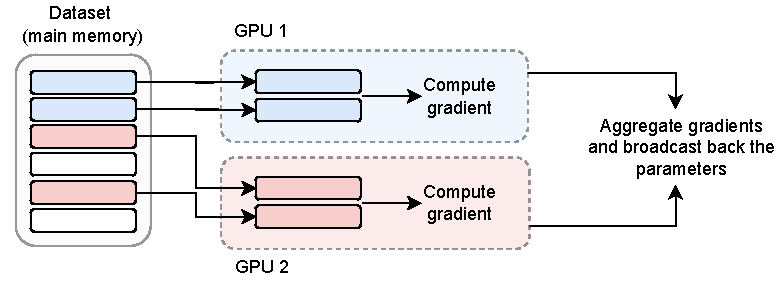
\includegraphics[width=0.7\columnwidth]{images/lecture_2/mini_batch.pdf}
		\caption{A simple form of distributed stochastic optimization: we process one mini-batch per available machine or GPU (by replicating the weights on each of them) and sum or average
			the corresponding gradients before broadcasting back the result (which is valid due to the linearity of the gradient operation). This requires a synchronization mechanism across the machines or the GPUs.}
	\end{figure}
	
\end{whiteframe}

\begin{frame}{Choosing the batch size}
	
	Running SGD requires selecting the size of the mini-batch, which is an additional hyper-parameter:
	
	\begin{itemize}
		\item Smaller mini-batches are faster, but the network might require more iterations to converge because the gradient is noisier.
		\item Larger mini-batches provide a more reliable estimation of the gradient, but are slower.
	\end{itemize}
	
	In general, it is typical to choose power-of-two sizes (32, 64, 128, ...) depending on the hardware configuration and the total memory available.
	
	In the limit $M=1$ we obtain an \myalert{online} (streaming) optimization. 
	
\end{frame}

\begin{frame}{Momentum}
	
	Steepest-descent directions are local. With noisy gradients, the resulting path can be erratic. As an example of a more advanced algorithm, \myalert{momentum} smooths the path by conserving some direction from the previous iteration:
	%
	\begin{align*}
		\vc{g}_t &= {\color{darkred}-\eta_t\nabla J(\vc{\theta}_{t-1})}
		+ {\color{darkpastelblue}\lambda\vc{g}_{t-1}}\,,\\
		\vc{\theta}_t &= \vc{\theta}_{t-1}+\vc{g}_t\,,
		\qquad \vc{g}_0=\vc{0}\,.
	\end{align*}
	
	The contribution from $n$ iterations ago is dampened by a factor $\lambda^{n-1}$. This remains an active research area (see, e.g, Adam, AdamW, Muon, ...).
	
\end{frame}


\begin{frame}{Definition of a convex function}
	
	\myalert{Convexity} plays a pivotal role in optimization. If a function is convex, its optimization is easier with respect to a non-convex one. 
	
	\begin{tcolorbox}
	$f$ is said to be convex if for any $\lambda \in [0,1]$:
	
	\begin{equation}
	f\Bigl((1-\lambda)\vc{x}_1 + \lambda \vc{x}_2\Bigr) \le (1-\lambda)f(\vc{x}_1) + \lambda f(\vc{x}_2) \,.
	\end{equation}
	\end{tcolorbox}
		
	If the equality is strict, we say that $f$ is \myalert{strictly convex}.
	
\end{frame}

\begin{whiteframe}{Convex vs. non-convex functions}
		
	\begin{figure}
	\centering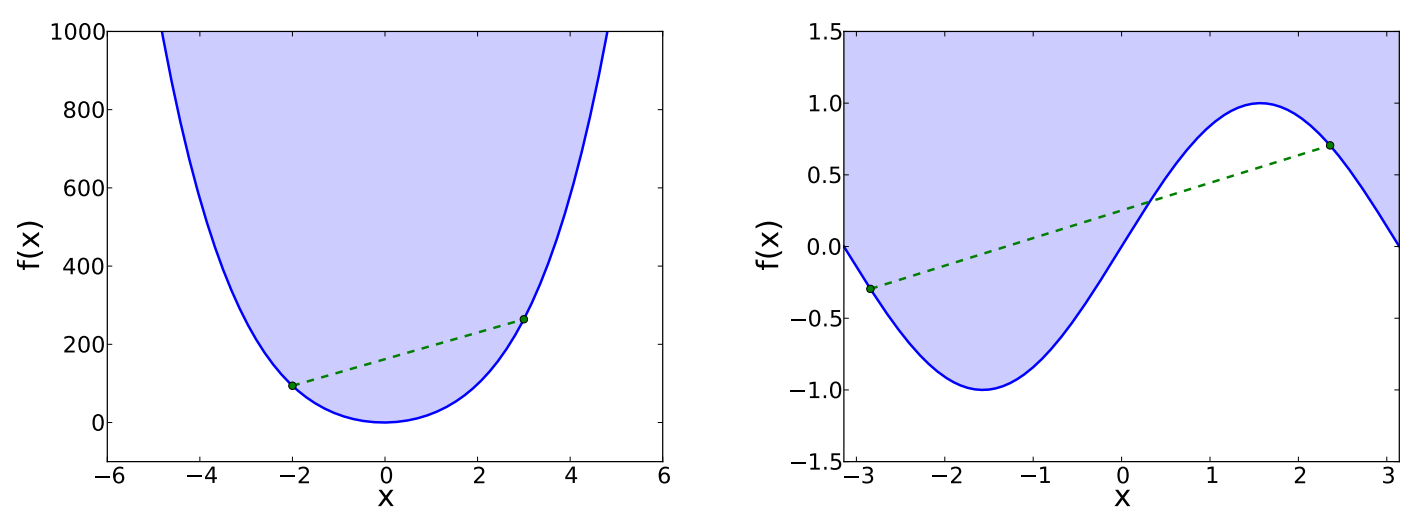
\includegraphics[width=11cm, keepaspectratio]{images/lecture_2/Convex_non_convex_functions.png}
	\caption{Left: an example of convex function. Right: an example of non-convex function. Taken from ``An Introduction to Machine Learning'' by Smola and Vishwanathan [unpublished].}
	\end{figure}
		
\end{whiteframe}

\begin{frame}{Notable results on gradient descent}
	
	\begin{tcolorbox}
	Consider a generic $J(\vc{\theta})$, and assume (S)GD converges to a point $\vc{\theta}^*$. Then:
	%
	\vspace{-1em}
	\begin{itemize}
		\item \textbf{Generic  non-convex $J(\vc{\theta})$}: The point $\vc{\theta}^*$ is \textbf{stationary}.
		\item \textbf{Convex $J(\vc{\theta})$}: The point $\vc{\theta}^*$ is a \textbf{global optimum}.
		\item \textbf{Strictly convex $J(\vc{\theta})$}: The point $\vc{\theta}^*$ is \textbf{the only} global optimum.
	\end{itemize}
	\end{tcolorbox}
	%
	For a non-convex function, unless additional assumptions are made on $J(\vc{\theta})$, this result cannot be improved. Finding a global optimum becomes an \textbf{NP-hard} problem, akin to evaluating the entire domain of the function.
	
\end{frame}

\begin{frame}{Reading material}
	
	\textbf{Chapter 2} from the book, along with the suggested exercises.
	
\end{frame}

\end{document}
